\documentclass{article}
\usepackage[a4paper, total={6in, 8in}]{geometry}

\usepackage{booktabs}
\usepackage{tabularx}
\usepackage{lipsum}
\usepackage{graphicx}

\title{Development Plan\\\progname}

\author{\authname}

\date{}

%% Comments

\usepackage{color}

\newif\ifcomments\commentstrue %displays comments
%\newif\ifcomments\commentsfalse %so that comments do not display

\ifcomments
\newcommand{\authornote}[3]{\textcolor{#1}{[#3 ---#2]}}
\newcommand{\todo}[1]{\textcolor{red}{[TODO: #1]}}
\else
\newcommand{\authornote}[3]{}
\newcommand{\todo}[1]{}
\fi

\newcommand{\wss}[1]{\authornote{blue}{SS}{#1}} 
\newcommand{\plt}[1]{\authornote{magenta}{TPLT}{#1}} %For explanation of the template
\newcommand{\an}[1]{\authornote{cyan}{Author}{#1}}

%% Common Parts

\newcommand{\progname}{Mechatronics Engineering} % PUT YOUR PROGRAM NAME HERE
\newcommand{\authname}{Team \# 34, ParkingLotHawk
\\ Fady Zekry Hanna, zekryhf
\\ Winnie Trandinh, trandint
\\ Muhammad Ali, alim102
\\ Muhammad Khan, khanm120} % AUTHOR NAMES                  

\usepackage{hyperref}
    \hypersetup{colorlinks=true, linkcolor=blue, citecolor=blue, filecolor=blue,
                urlcolor=blue, unicode=false}
    \urlstyle{same}
                                


\begin{document}

\begin{table}[hp]
\caption{Revision History} \label{TblRevisionHistory}
\begin{tabularx}{\textwidth}{llX}
\toprule
\textbf{Date} & \textbf{Developer(s)} & \textbf{Change}\\
\midrule
September 27, 2022 & Winnie Trandinh & Added Sections 1 to 4\\
September 27, 2022 & Fady Zekry Hanna & Added Sections 5 to 8 and added final touches\\


\bottomrule
\end{tabularx}
\end{table}


\newpage

\maketitle

\indent Existing solutions sometimes involve a designated person, a parking lot officer, who helps to communicate parking spot availability to visitors. Of course, the primary drawback is that the operator being a person often cannot see or monitor large swaths of the parking lot accurately. Other solutions involve installing vehicle counters in the parking lot. These vehicle counters are installed either at the entrance/exits or throughout the parking lot, such as a distributed system of cameras.  These solutions are expensive and involve installations at precise locations, and thus require greater investment for organizers. Vehicle counter technology thus does not fulfill the need for many outdoor, seasonal, temporary, and/or cheaper organizers.  Examples include provincial/national parks, concerts, and religious places of worship where the highest demand for this solution is only for a certain period of time. 
\subsection{Project Description}

ParkingLotHawk is an aerial drone that will fly above the parking lot to gather information about slot availability and general parking lot status. The parking lot authorities will be able to access and visualize this information from an application on their Personal Computers (PCs). The parking lot authorities will command the ParkingLotHawk  only through an application running on their PC. The drone will be able to stabilize and move to different locations autonomously. Thus from the PC application, the operator will be able to launch or land the drone, after which they can either let the drone mutinously investigate the entire parking lot or have the drone investigate specific sections of the parking lot. 

\section{Team Meeting Plan}

Meetings for the team will be conducted on a weekly basis, on Thursdays at 2:30pm. The default meeting location will be at Thode Library, unless explicitly specified otherwise. Additional meetings and work sessions will be arranged if required and will be determined by the team. 
\\
The meeting roles are provided in Table 2.
\begin{table}[!h]
\begin{center}
\caption {Team Meeting Roles} \label{tab:title}
\begin{tabular}{ | m{2cm} | m{2cm} | m{8cm} | }
\hline
 Role & Name & Description \\ 
 \hline
 Chair & Ali & The chair is responsible for leading the meeting. The chair will further be responsible for transitioning between agenda items and ensuring that the agenda item does not exceed its allocated time.   \\  
 \hline
 Scribe & Ali & The scribe is responsible for taking meeting minutes if required, and clearly documenting the required action items at the end of each meeting. \\
 \hline
 Member & Fady, Ali, Zaid, and Winnie & All members are responsible for adding agenda items for the meeting, leading discussions on their domain of expertise, and ensuring that they are prepared for each agenda item prior to the meeting. \\
 \hline
\end{tabular}
\end{center}
\end{table}

Meetings will be conducted through the use of an agenda and will be kept under one hour in length. A day prior to the meeting, all members are responsible for creating a completed agenda which contains the discussion items and the allocated time to spend on it. Potential discussion items include design considerations and important issues and should be phrased as questions to promote discussion amongst the team. These items should then be led by either the member with the relevant expertise or by the creator of the item.  

From the period between the meeting date and one day prior, all members are responsible for gaining knowledge on all the agenda items such that they are prepared for insightful discussions during the meeting. During this period, special consideration will also be given to new agenda items that were not previously created if the team agrees that the item is time sensitive. 

During the meeting, all members are expected to be present and give relevant input to the agenda items. The leader for the meeting will transition from the Chair and the leads for the agenda item, as previously determined. All agenda items will be kept within the allocated time, and if the need arises for a longer discussion, an additional meeting will be organized at a later date. The result of the meeting will be a list of action items written by the Scribe that the team must partake to address issues raised within the meeting, in addition to a short summary of the decisions agreed upon during the meeting. 

\section{Team Communication Plan}

The success of the team depends on great communication. The team has come to a consensus to use Git Issues for issue tracking, which will then be integrated into MS Teams using the GitHub Bot available on Teams. Git Projects will be used for project and task management amongst team members. For the main method of communication, all team members will use the created MS Teams chat and channel, with the Teams channel having separate topic subchannels. OneNote and Microsoft Word will be used for written documents and scribble for the design and documentation process. Team members have also exchanged phone numbers and emails in case of emergency.  

\section{Team Member Roles}

The team is composed of two main administrative roles: the Team Leader and the Scribe. Externally, the Team Leader is the main point of contact between the team and stakeholders, and internally is responsible for organizing and managing the team. Such tasks include team restructurings, settling disputes, and promoting teamwork. The Scribe is responsible for recording major decisions within the team, both during team meetings as described in Team Member Meetings, and also during unofficial discussions that may arise.  

The team also includes various domain experts relevant to the project. These experts are then responsible for their domain, and issues and integration within that domain will be handled by the expert. This allows for distributed responsibility and knowledge of the project, and collectively ensures that detailed knowledge about a particular domain is present within the team. 

For many of the technical domains, the team has opted to partake in a dual-expert system where two experts are present for the domain. This ensures that in the absence of an expert, the effects on the team are minimized. Furthermore, this promotes collaboration between the experts during their research of their domain. 

The team has also defined what it means to be an expert in their domain: 
\begin{itemize}
    \item In depth understanding of how the component works physically (if applicable). 
    \item Proper reasoning as to why specific component/firmware was chosen.
    \item In depth understanding of the key parameters and specifications of the product/firmware.
    \item In depth understanding of the inputs and outputs to the domain. 
    \item In depth understanding of the integration of the domain into the project. 
\end{itemize}

The list of domains along with the assigned experts are outlined in Table 3.
\\
\begin{table}[!h]
\caption {Assigned Experts} \label{tab:title}
\begin{center}
\begin{tabular}{ | m{3cm} | m{3cm} | m{8cm} | }
\hline
Domain & Assigned Experts & Description of Domain \\
\hline
Documentation & Zaid & The documentation domain includes the written documentation for the development process, design considerations, and any other resources that are helpful to the team. \\
\hline
Git & Ali & This domain is responsible for managing Git and its related features, including version control, issues maintenance, and merges.\\
\hline
Latex & Zaid & The Latex domain expert is responsible for understanding the Latex syntax and generation process. \\
\hline
Power Management and Motors & Fady and Zaid & This domain relates to the powering of the individual components of the drone, and the control of the motors. Example components include the battery, Power Distribution Board, and the Electronic Speed Controller. \\
\hline
Mechanical Design & Winnie and Ali & Included within this domain is the creation of the custom drone frame, in addition to minimizing vibrations while maximizing structural integrity. \\
\hline
External Sensors and Peripherals & Winnie and Ali & This domain includes the external sensors that connect to the flight controller, including the camera, radio transmitter, and any other sensors that may be required. \\
\hline
Flight Controller & Zaid, Fady, Ali, and Winnie & All the members should be responsible for being experts at the Flight Controller as they all need to know how to interface with it. Further sub domains may be created at a later date if the need arises. \\
\hline
Internal Sensors & Winnie and Ali & The Internal Sensors domain includes the sensors within the Flight Controller. Such sensors include the Inertial Measurement Unit, barometer, and GPS. \\
\hline
\end{tabular}
\end{center}
\end{table}

The domains of expertise will dynamically evolve with the progression of the project to ensure that newer relevant domains are added. For example, the current development focus is hardware heavy, which leads to multiple hardware related domains. Once the construction of the drone is completed, software domains will play a larger factor in the development of the project, thus creating new domains with new experts. Such new domains may include ‘Software in the Loop Simulations’ and ‘Localization and Mapping’. If the need for role switching arises, the member(s) switching must provide written record that they agree to said switch, and they are responsible for any knowledge transfers that may be required. However, unless a valid reason is provided, roles will remain the same to prevent the need for detailed knowledge transferring. 
\newpage

\section{Workflow Plan}

The team will use GitHub as the primary software for source control and tracking the project development, through the usage of a Feature-Branch methodology. The project will consist of a Master branch, in which the code has passed all unit test cases and linter errors. Development of new features will be branched off the Master branch, with a descriptive branch name that states the feature being developed. Further commits on this feature branch shall follow a two-part commit message format. The first part of the message will clearly state what changes were made within the commit, whereas the second part will give the rationale as to why the change was required. Once the feature is completed, a pull request (PR) will be made into the Master branch at which point unit tests and integration tests will be automatically conducted through the use of Continuous Integration (CI). Upon successful completion of the tests, the PR will be verified by at least 2 other members before the branch is merged into the Master branch.  

To assist in the development of the project, GitHub Issues will be used to document all technical and design related tasks and can be created by any member. These issues will then be linked to the tasks within GitHub Projects, which is the chosen project management software, thus enabling the automatic issue closure once the task is set to completed as well as increasing the ease of issue traceability. To further organize the issues, predefined tags will be used to sort the issues by their domain and importance, with one or more labels present in each issue. These labels are described in in the table below. 

\begin{table}[h]
\caption {Git Issue Labels} \label{tab:title}
\begin{center}
\begin{tabular}{ | c | l | }
\hline
Label & Description \\
\hline
Documentation & Issues pertaining to incorrect or missing documentation. \\
\hline
Sensors & Issues concerning sensor interfacing or integration. \\
\hline
Design & Issues regarding the physical or software design of the product. \\
\hline
Software & Issues concerning the software functions of the product. \\
\hline
Quality of Life & Issues that are not required to be fixed but may help in the future. \\
\hline
High Priority & High priority issues that must be fixed as soon as possible. \\
\hline
\end{tabular}
\end{center}
\end{table}

Predefined milestones will also be used within the team to coordinate periodic releases of the product. These milestones are outlined within the Project Schedule section and provides the general development path for the project. Once the milestone is reached on the Master branch, a Project Release and Git Tag will be made from the Master branch. This serves as a record of the product at all major points of its development and increases the traceability of new bugs, as the introduction of major components can be precisely determined from the release history. 

\section{Proof of Concept Demonstration Plan}

The risks of building an aerial drone from scratch without a flight controller are countless. Imagine trying to develop a drone that consistently wobbles during flight and trying to root cause the multiple variables that contribute to the issue. The variables could be gyroscope, accelerometer, and barometer calibrations, controls design setup, or environmental variables like wind speed. Developing an aerial drone using sensors and a microcontroller is possible but beyond the scope of a capstone project. A flight controller that has the required sensors integrated for flight allows the group to further develop the minimum viable product mentioned within the Goals document. 

The team has researched multiple flight controllers and decided to proceed with the \href{https://navio2.emlid.com/}{Navio2 flight controller}. The flight controller is well documented online, with a dedicated forum for aerial drone enthusiasts.  The available documentation online allows the group to quickly find solutions to any issues during the process of building the drone
\subsection{Sensor and Serial Communication}
The most significant risk is losing sensor and motor communication midflight. Before trying to fly the drone, the group plans on testing the motors without propellers attached and moving the flight controller in an infinity figure motion to ensure the adequate functionality of the sensors. Doing so allows the group to unit test the individual components and determine any issues and root cause problems in a safer manner.

\subsection{Drone Specifications}
Drone frame dimensions, motor stator and constant velocity, the propeller diameter, and battery size are all vital specifications that need to be considered. Having one of these variables not adequately set can cause in a loss of resources and non-flyable drone.

To ensure compatibility between the components, the will follow standard guidelines on the required specifications of the components, in relation to the frame size. This will ensure that enough lift is generated for the drone size, and adequate power is supplied to the electrical components.

\subsection{Drone Lift}
The lift of a drone can be challenging. The challenges the group anticipates overcoming are the weight of the system, the chassis weight distribution, and the vertical propulsion in the workspace. To mitigate these challenges, the group plans on testing the drone in an enclosed working space while limiting the altitude of the drone. The group will inspect the behaviour of the drone within controlled variables and make the necessary changes accordingly.

\subsection{Drone Landing}
 To limit the shock of landing, the group will design landing rods that will absorb landing shock. The rod will be something similar to the rods in the image below.\\


\begin{figure}[h!]
  \begin{center} 
  \caption{Drone landing rods example} 
 
        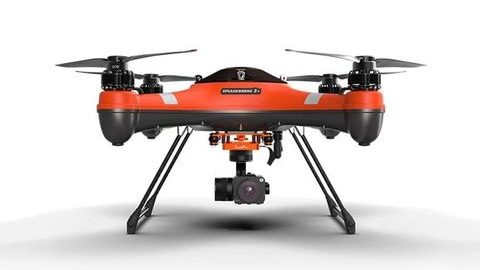
\includegraphics[width=0.5\textwidth]{drone.jpg}
  \end{center}
\end{figure}


\section{Technology}
There are several key hardware and firmware components that will need to be purchased, integrated and tested before advanced algorithms can be developed and tested.  
\begin{itemize}
    \item Frame - A custom fabricated frame. This will house all of the other drone components.
\item Solidworks - 3D Design software used for the design of the frame
\item Brushless Motors
\item Propellers
\item Navio2 Flight Controller- Physical flight controller hardware, contains various sensors such as barometer, hyroscope, accelerometer, GPS, etc. Other electrical components, such as the motores and baterries will interface with this Navio2. 
\item Batteries
\item Camera - placed on drone
\item Raspberry Pi (RPi) - Physical board placed on the drone. Runs various algorithms and controls the execution of the Navio2. 
\item Radio - used to send commands to the flight controller and raspberry PI
\item ArduPilot - Flight controller firmware, will be flashed and run on the Navio2. This software will run control the motors based on the sensor reading within the Navio2. This software contains tuning parameters that will be tuned during testing.
\item Power Distribution Board - circuit board which transfers appropriate amounts of voltage to each electrical component, such as the battery, ESCs, Flight Controller and Motors. All electrical components receive power from this board. 
\end{itemize}


Once the drone is able to fly reliably and accurately, software modules and algorithms will be developed. Heavy image processing algorithms are run on the RPi. Control algorithms to move and land the drone in various locations are also run on the RPi.
• Python: Used for prototyping the first software versions of the image and control algorithms. Python will also be used to develop the user interface for the Operator. 
\begin{itemize}
    \item C++: C++ will be used to write image and control algorithms.
\item Clang-Tidy - C++ linter.
\item Pylint - Python linter.
\item Visual Studio Code: will be the IDE for python, and the text editor for C++.
\end{itemize}


The algorithms will be developed and tested on various kinds of test. Different types of testing may require specific technology.
• Unit testing - Bench testing of individual components will be done before integration with the drone. Basic functionality with the flight controller (ability to turn on, follow commands, and stay on) will be verified. 
\begin{itemize}
    \item Unit testing - Bench testing of individual components will be done before integration with the drone. Basic functionality with the flight controller (ability to turn on, follow commands, and stay on) will be verified. 
    \item Indoor Drone Testing - Will be done to ensure basic flying capabilities before outdoor testing. A large transparent cube will be created to ensure safety of the developers.  
    \item Safety Glasses  and First Aid Kit for safety
    \item Simulation Testing - Software for the simulation of the quadcopter (ArduPilot's Software-in-the-loop, (SITL)) is provided by the firmware, allowing for code execution of a simulation target. Once the drone is able to fly, any extra control algorithms and localization algorithms will be developed using this framework in addition to a simulation visualizer tool, such as Gazebo and Simulink. 
\end{itemize}


Overleaf will be used for document generation from Latex.


\section{Coding Standard}
To ensure consistency in code within the team, all members will use VS Code as the Integrated Development Environment (IDE), with a maximum code length per line of 150 characters and the linter enabled. As linters are language specific, the chosen linters are Pylint for Python and clang-tidy for C++. To further improve consistency between the team, as well as between languages, the team will be using the Drake Style Guide. 

To use consistent naming conventions, the team will be following camel case rules and has opted to use affixes as stated below in in the table below.

\begin{table}[h]
\begin{center}
    

\caption {Variable Affixes} \label{tab:title}

\begin{tabular}{ | m{4cm} | m{4cm} | m{4cm} |} 


    \hline
     Affix Type & Affix & Variable Type\\ 
 
    \hline
     Prefix & \texttt{m\_}& Member variables\\ 

    \hline
     Prefix & \texttt{g\_} & Global variables\\
     
     \hline
     Suffix & \texttt{\_e} & Enumeration variables\\
     
     \hline
\end{tabular}
\end{center}
\end{table}


Within the Github repository, all members will abide by a two-part commit message format, as described in the Project Workflow section in addition to linking all pull requests with an issue. This further improves consistency between the members, as well as increasing the traceability of tasks.








\section{Project Scheduling}
There are two levels of project scheduling, one being the day to day agenda which tries to follow ad meet the higher level, long term schedule. The long-term schedule consists of a  list of milestones the team has collectively agreed on. 





\begin{table}[h]
\begin{center}
    

\caption {Milestone Dates} \label{tab:title}

\begin{tabular}{ | m{2cm} | m{11cm} | } 
\hline
Date & Task\\

\hline

October 2 &
\begin{itemize}
    \item Finalize and order drone component
    \item Send out finalized 3D models to McMaster 3D printing facility, the whole print will likely take weeks.
\end{itemize}   \\

\hline
October 5 & Finalize, order, find and/or create safety related equipment in preparation of flight tests, such as safety glasses and transparent cube.\\

\hline
October 25 & Setup the simulation environment while the parts have not arrived.\\
    
\hline
November 2 & Verify that IMU on flight controller is giving accurate readings to the ArduPilot firmware. This verifies that the flight controller and firmware is communicating.\\

\hline
November 6 & Verify that the flight controller is able to spin the motors. This step confirms most several key hardware pieces are functioning correctly: battery, power distribution board, Raspberry Pi, flight controller, ESC's, and motors. This step will likely reveal issues with the ordered hardware, and is thus best performed early. \\

\hline
November 10 & Integrate the pieces of the drone onto the frame. \\
\hline
November 13 & Present the proof of concept.\\

\hline
November 22 & Verify that the radios and cameras are able to connect to the Raspberry Pi.\\

\hline
December 2 & Tune the flight controller to the point that the drone can stabilize and maneuver. This will likely start with getting the drone to first lift off, then to hover, to land safely and finally to aerially move to specific location GPS locations. \\

\hline
December 20 & Create a user application to receive live camera output. This application will be used by parking lot operators.\\

\hline
January 1 & Collect some live video from the drone on parking lots. This data will be used to test vision and parking lot algorithms developed later on.\\

\hline
January 15 & Develop the feature that allows the operator to command the drone to a specific GPS location.\\

\hline
January 30 & Develop the vision/perception algorithm that lets the drone know when the parking lot ends, and the control to prevents the drone from exploring beyond parking lot boundaries.\\

\hline
February 1 & Version 0, minimum viable product demonstration. \\

\hline
February 15 & Develop the algorithm to make the drone autonomously fly over every section of an irregularly shaped parking lot. \\

\hline
March 1 & Develop and test the algorithm to take off and land at multiple points in and around the parking lot. \\

\hline
March 15 & Develop an algorithm to create an occupancy map of the parking lot. \\

\hline
April 1 & Iteratively develop and test the computer vision and control algorithms in order to meet the specified the stretch goals. The algorithms can be tested using real videos collected in previous steps or using the simulation environment.\\
\hline

\end{tabular}
\end{center}
\end{table}

These large milestones will be broken down into sub-tasks. The sub-tasks will be documented on Git Issues and Git Projects, and a task priority will be included. Breaking these milestones down into modules is a task that the team will do together after a given milestone is completed. 

Our team plans on using Projects feature on GitHub to track the progress of these Git Issues. This is convenient as this means all short term project management will be done on a single website. Additionally, it also allows to keep track and work on the task at the same time during the entirety of this project.

When it comes to assigning the Git Issues among the team members, they will be assigned based on the roles that were determined for each individual earlier. In order to manage the resources in the team, it is assumed that each member will spend 9-12 hours per week on the project, and will be assigned issues according to this constraint.


\end{document}